\chapter{Computational physiology}
\label{sec:models}
A mathematical formalization of the fundamental knowledge and relation among biological system - mathematical model - is used as a base abstraction to utilize current discoveries of the genomics and proteomics and formalize the knowledge and construct a "Physiome Model". Model by it's definition is simplification of the complex reality.

Constructing the models and integrating them into complex entity which can be used for further purposes is schematically illustrated in fig. \ref{fig:modeling}. The measurements are done in laboratories or in hospitals. Lumped parameter models are usually represented as ordinary differential equations and differential algebraic equations and characterize the reality as topology of discrete elements. The imaging methods for processing and analysis (section \ref{sec:imaging}) are used to construct 3D models from segmentation and generating of mesh representation connected to physical principles. 
\begin{figure}[ht]
    \centering
    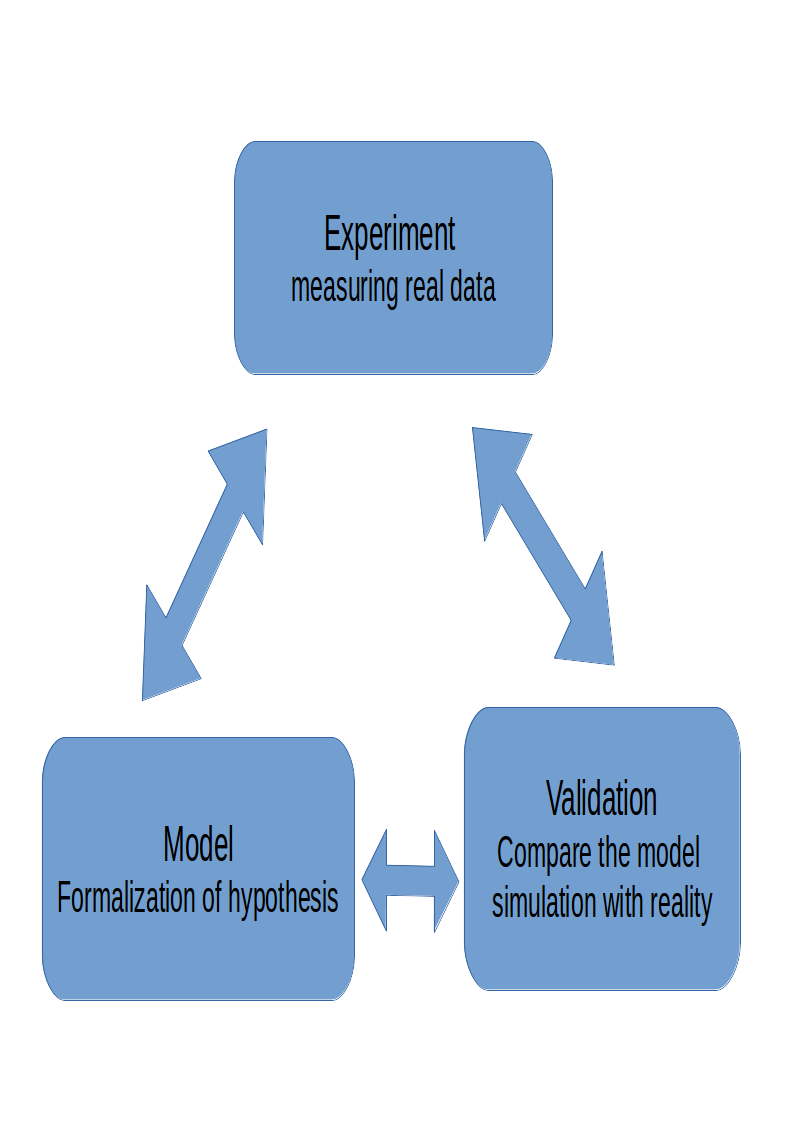
\includegraphics[width=0.5\textwidth, height=5cm]{chapter6/modeling.png}
    \caption{Schematic illustration of scientific process. The experiments produces data which are interpreted and hypothese is formalized as a model. Validation compares the model simulation with experiment, if model satisfies the criteria - is in agreement with real experiments, then the validated model can be used for other purposes.  %\bibentry{EGICompendium2013} \bibentry{egi2014}.
    }
    \label{fig:modeling}
\end{figure}

Application of the mathematical modelling techniques towards the biomedical research is sometimes called as systems biology approach combining the reductionism and integration as denoted by Kohl et al.\cite{Kohl2010}. Application towards the clinical praxis include the quantification of the diagnostic index or treatment strategy and it is a goal to develop tools, database models and methods of several Physiome projects, e.g. VPH-Physiome project presented by Hunter et al.\cite{Hunter2009}.

One of the earliest complex and integrative modelling effort was a model of circulation and it's regulation published by Guyton et al. in 1972 \cite{Guyton1972} which via derivative and technological upgrade continues as "Human Model" or "HumMod" introduced by Hester et al. \cite{Hester2011systems,hester2011} with a focus on integration effort. Different approach of modelling human physiology is a database of smaller models focusing on some particular physiological phenomenon. E.g. the NSR Physiome project introduces  JSIM\footnote{JSIM: \url{http://www.physiome.org/jsim/} accessed January 2015} Java based simulation system to support modeling in  physiology. Repository of several hundred of models were published using this system \cite{Butterworth2014}. The similar effort is done by IUPS Physiome project and repository of models are  based on XML standard languages CellML and FieldML \cite{Hunter2004,Yu2011}. The Systems Biology Markup Language (SBML) is used for modeling biological system at the level of biochemical reaction and regulatory network and another database collects several hundreds of curated and non-curated models \cite{Hucka2004,LeNovere2006}.

JSIM, CellML, SBML or HumMod are domain specific languages and the tools able to work with them are primarily developed within physiological or systems biological communities. Other authors use commercial or industry standard tools for mathematical modelling and computing. E.g. Kofranek et al. describes Guyton's 1972 model in MATLAB\textsuperscript{\textregistered} Simulink \cite{Kofranek2010} and the derivative HumMod in acausal object-oriented Modelica language \cite{Kofranek2011hummod,kofranek2013hummod}. Fernandez et al. describes models of cardiovascular pulsatile system using MATLAB Simscape  \cite{FernandezDeCanete2013} and recently in Modelica  \cite{FernandezdeCanete2014}.

Thus there is an open debate whether in-house domain specific language and tools like JSIM, CellML and FieldML,SBML or HumMod reached it's capabilities for representing complex models. Only the HumMod reached the integrative approach building the complex integrative model of human physiology using lumped parameter approach. I contributed to the idea of key features which involves acausal modeling technique and object orientation which keeps the complex model structure decomposed into understandable and maintainable parts and allows to cover complexity of models like HumMod. 

The methods and examples of modeling cardiovascular system are described in the next section \ref{sec:methodsmodels}. The methods of estimating parameters of complex models are described in section \ref{sec:methodsestimation} and particular results are described in section \ref{sec:resultsestimation}.

%\label{sec:results}
\section{Modeling methodology}
\label{sec:methodsmodels}
%For building complex models it seems that acausal (or declarative) modeling technique is key feature as it allows to express the variables declaratively, acausal modeling tool (e.g. Modelica or MATLAB\textsuperscript{\textregistered}  SIMSCAPE\texttrademark) figures out which are the dependent and independent variables upon compilation\cite{fritzson2002}. This allows building complex systems of equation from composed components and the model diagrams still captures the essence of the modeled reality much better and the simulation models are much more legible and thus also less prone to mistakes\cite{Kofranek2008,FernandezDeCanete2013}. 
The methodology of formalizing mathematical models is influenced by the abilities of underlying modeling language used. %As it was noted in previous chapter \ref{sec:intromodels}, the technology used for formalizing mathematically knowledge may introduce some benefits.
%\subsection{Modelica}
The Modelica language is an object-oriented, equation based and acausal modeling language standardized by Modelica association\footnote{\url{http://www.modelica.org} accessed February 2015}.

Object orientation means that the definition of model is class as in object oriented programming, instance of the model is object,  each instance can share type and differ in parameters and the place where it is used, inheritance and some sort of polymorphism is possible.

Equation based means that the equation is not statement, thus the relation among variables can be expressed in any form. Modelica tool will decide which one is input and output upon compilation. E.g. from the equation $q = \frac{dV}{dt}$ the process of computation can lead to $ q:= der(V)$ or $ V := \int{q}dt$ based on whether the $V$ or $q$ is known from the context.

Acausal connector is special purpose class to define variables of the model shared with other models or classes. Connecting two or more components via acausal connector will generate equality of all "non-flow" variables in connected connectors: $$p_1=p_2=\ldots =p_n$$
and zero sum of all "flow" variables $$ \sum_{i=1}^n q_i=0$$

%As an example, we will declare components important for modeling cardiovascular system (CVS). The components are hydraulic elastic ballon, which is analogy of electrical capacitor, and hydraulic resistor, analogy of electrical resistor.
%
%Connector \emph{HydraulicPort} with "flow" variable $q$ and non-flow variable pressure $p$ is presented in Modelica source code:
%\begin{lstlisting}[language=modelica]
%connector HydraulicPort
%  flow Real q;
%  Real p;
%end HydraulicPort;
%\end{lstlisting}
%
%Model of hydraulic resistor(conductor) with parameter $G$ denoting conductance and two hydraulic ports express the equations:
%\begin{equation}
%q_{in}.q = -q_{out}.q \label{eq:conductor1}
%\end{equation} 
%\begin{equation}
% q_{in}.q = G \times (q_{in}.p-q_{out}.p) \label{eq:conductor2}
%\end{equation}
%presented in Modelica source code:
%\begin{lstlisting}[language=modelica]
%model HydraulicConductor
%  parameter Real G;
%  HydraulicPort qin;
%  HydraulicPort qout;
%equation 
%  qin.q= -qout.q;
%  qin.q = G*(qin.p-qout.p);
%end HydraulicConductor;
%\end{lstlisting}
%
%
%Model of hydraulic elastance with parameters $V_0$ as unstressed volume $p_0$ external pressure and $C$ compliance(reciprocal value of elastance) with state variable $V$ volume express these equation:
%\begin{equation} \label{eq:compliance}p-p_0 = \left\{   
%  \begin{array}{l l} 0 & \quad \text{if } V \text{\textless} V_0 \\ 
%    \frac{V-V_0}{C} & \quad \text{otherwise}
%  \end{array} \right.\end{equation} 
%\begin{equation}\label{eq:flowrate}\frac{{\rm d}V}{{\rm d}t} =  q\end{equation} 
%is presented in Modelica source code:
%\begin{lstlisting}[language=modelica]
%model HydraulicElastance
%    Real V;
%    parameter Real V0;
%    parameter Real p0;
%    parameter Real C;
%  HydraulicPort qin;
%equation 
%   qin.p -p0 = if (V<V0) then 0 else (V-V0)/C;
%   der(V) = qin.q;
%end HydraulicElastance;\end{lstlisting}

The paper \cite{Kulhanek2014Modeling} \emph{Modelling of Short-term Mechanism of arterial pressure in the cardiovascular system: Object-oriented and acausal approach} in Appendix~\ref{app:d} published disputation about causal and acausal approach in using Modelica for modeling lumped parameter CVS model. 

The paper \cite{Kulhanek2014mefanet} \emph{Simple Models of the Cardiovascular System for Educational and Research Purposes} in Appendix~\ref{app:simplemodelsd} published detailed methodology of modeling pulsatile CVS in Modelica. 

Comprehensive guide to the Modelica language and it's capabilities are in the book of Fritzson \cite{fritzson2002} or in the on-line book by M.Tiller \cite{Tiller2014}.

\section{Parameter Estimation}
\label{sec:estimation}

%\subsection{Identification of physiological systems}
%Model verification (whether simulation of the model shows desired behavior) and model validation (whether model simulation agrees with new observation of real system) are important steps in system analysis and model construction. 
Usually some knowledge of the system - the structure is available and unknown coefficients (parameters) remain unknown. Once the model is formalized and constructed, further problem is to estimate the model parameters so that the model reproduces real world system. This procedure is sometimes called model identification \cite[p.~159]{khoo2000}. The objective of this task is usually to minimize the following function (to find least squares of the differences between predicted and measured values):
\begin{equation} \label{eq:parameter} 
f( \vec{p} ) = \sum_{i=1}^{n} ( M(t_{i},\vec{p} ) - d(t_{i}) )^2 \to min  
\end{equation} 
where $\vec{p}$ is vector of values of parameters, $M(t_{i},\vec{p})$ is model simulated at time $t_{i} $ with the given parameter values $\vec{p}$ and $d(t_{i})$ is the measured experimental value at time $t_{i}$.
Algorithmically, this problem was shown to belonging to the \emph{NP-complete} problems \cite{Hofmann2005} thus the best exact algorithm is based on brute force search - trying all possible values of parameters and simulate the model with them and find minimum of the objective function \ref{eq:parameter}. 
However, exact solution may not be needed because the models itself are by definition approximation of real system, and the input data are measured with some degree of error. 
As in other problems where exact algorithm uses brute-force search, some heuristic or randomization method should be used for bigger space of potential input data. 
After the parameter estimation a further problems arise with structural identifiability and analysis of sensitivity to the estimated parameter values\cite[p.~176]{khoo2000}. 

Parameter estimation and further analysis methods are part of specialized mathematical software. E.g. Pruet et al. used Metropolis algorithm to produce a distribution of parameters to calibrate the model of human cardiovascular physiology, which were further tested against predictive ability of circulatory failure and statistical methods performed in the software Wolfram \textit{Mathematica} \cite{Pruett2013}. The iterative improvement method in the software MATLAB Simulink\textregistered ~was used in estimating 2 parameters of simple cardiovascular model by Takahashi et al. \cite{Takahashi2013}. Several methods were compared in estimating multiple parameters of cardiovascular system in MATLAB Simulink\textregistered ~by Abbass et al. \cite{Abbass2012}.

Heuristic methods reduce the number of simulation and additionally some set of  simulation can be computed concurently e.g. in grid or cloud computing infrastructure. 
Maffioletti et al. published GC3Pie framework utilizing evolutionary algorithms and introduced workflow to identify parameters of models for economical predictions using grid computing \cite{maffioletti2012computational}. Humphrey et al. calibrated hydrology models utilizing commercial Windows Azure cloud computing infrastructure with a significant speedup on the modified dynamically dimensioned search algorithm\cite{Humphrey2012,Tolson2007}. 

%Selected methods to estimate parameters are introduced in section \ref{sec:methodsmodels}. 

As already identified also by other authors of some calibrating systems, the parameter estimation is used sporadically, however, with high demand of computational task in temporal time. Thus, I proposed and designed the system which can distribute the simulation task into grid-computing and cloud-computing infrastructure and the computational capacity can be provisioned on-demand.% this brings significant speedup for parameter estimation of complex model but limited speedup on simple models. 
Methods are described in section \ref{sec:methodsestimation} and interesting results are described in section \ref{sec:resultsestimation}.

\section{Methods for Parameter Estimation}
\label{sec:methodsestimation}
Evolutionary algorithms are used for finding global minimum or maximum and it can be used to estimate the parameters of the model. Genetic algorithm is type of evolutionary algorithm and the general structure of the algorithm is presented in figure \ref{fig:GA-kopenogram}.

\begin{figure}[htb]
    \centering
    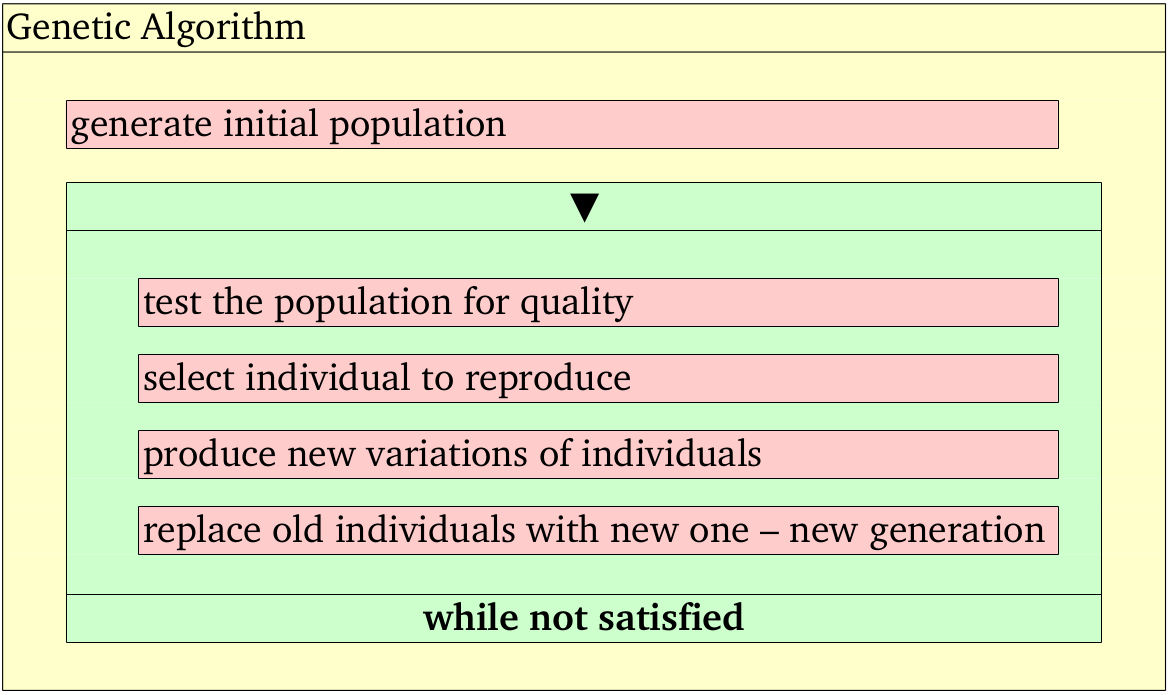
\includegraphics[width=0.6\textwidth]{chapter6/GA-kopenogram.png}
    \caption{General structure of genetic algorithm presented as kopenogram. Kopenograms are graphical language for structured algorithms to supplement UML proposed by Kofranek et al.\cite{Kofranek2012}.
    }
    \label{fig:GA-kopenogram}
\end{figure}


\begin{figure}[htb]
    \centering
    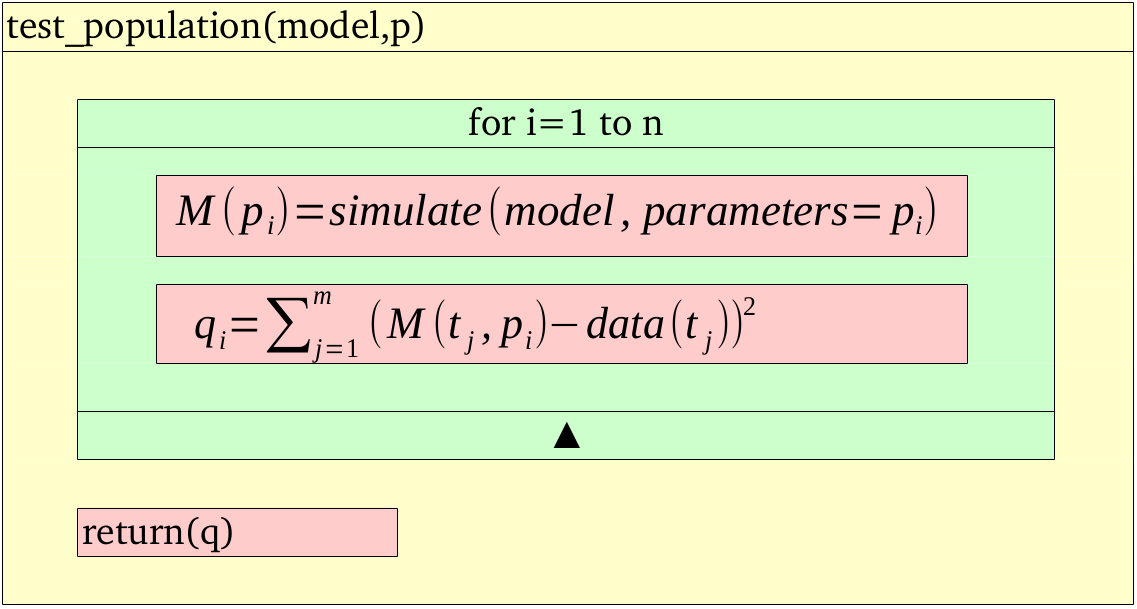
\includegraphics[width=0.6\textwidth]{chapter6/GA-kopenogram2.png}
    \caption{Specific test of the population for quality in case of parameter estimation. Model is simulated according to individual $i$ with parameters $p_i$ and the quality $q_i$ is counted per the objective function \ref{eq:parameter}.
    }
    \label{fig:GA-kopenogram2}
\end{figure}

The iteration within the loop "$\blacktriangledown \ldots$ \emph{while not satisfied}" depends on previous iteration, thus in general it cannot be parallelized.
In the case of parameter estimation, the step \emph{test the population for quality} has algorithmical structure as in fig.\ref{fig:GA-kopenogram2}. Each iteration in the loop "\emph{for i=1 to n}" is independent and a therefore loop parallelism (section \ref{sec:parallelprogramming}) can be utilized and implemented here.

The Amdahl's law in equation \ref{eq:amdahl} can be used to estimate  the theoretical speedup limitation for the specific model and potential gain for identifying different types of models can be stated. We assume that the simulation of the model with any parameters will take the same time, even this is not generally true as the non-linear models and numerical methods may cause different steps to be performed for different parameter values. 

The specific fraction $\alpha$ for the model determines the level of scalability of the model within the parallelized system. For the complex models the $\alpha$ will decrease. The specific estimates of the fraction $\alpha$ and it's influence on the scalability and results are presented in section \ref{sec:resultsestimation}.

\subsection{Architecture of system for parameter estimation}

The architecture of the system implementing the algorithms in fig. \ref{fig:GA-kopenogram} and \ref{fig:GA-kopenogram2} will determine the overhead which may affect significantly the computation time.

The architecture of the proposed system is in fig \ref{fig:architectureestimation}.
\begin{figure}[htb]
    \centering
    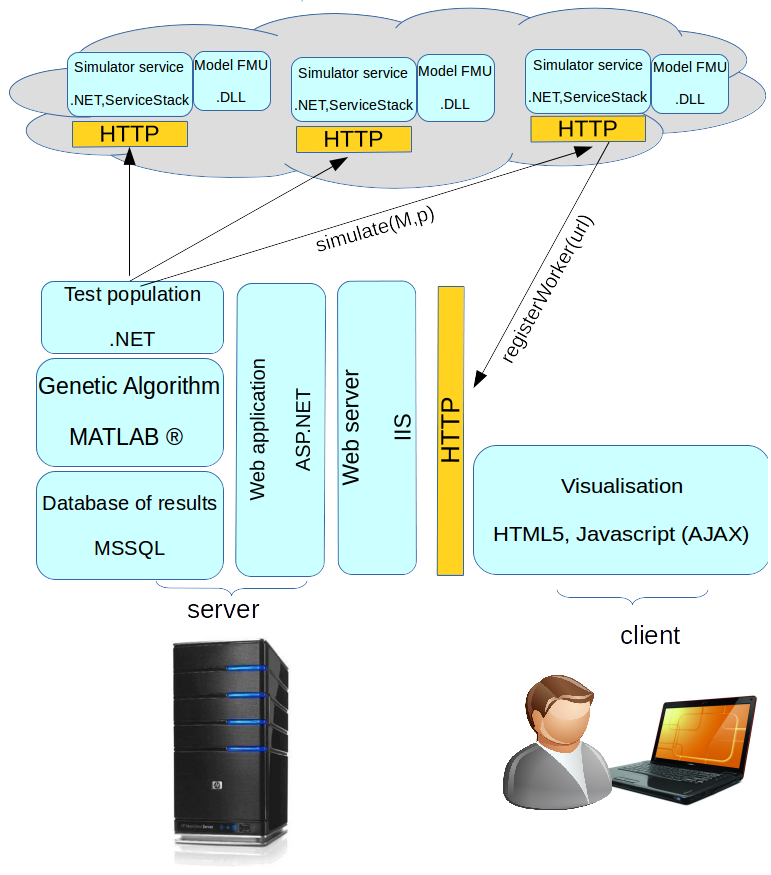
\includegraphics[width=0.6\textwidth]{chapter6/architekturaestimation.png}
    \caption{Architecture of the system employing genetic algorithm and concurent simulation of models in cloud.
    }
    \label{fig:architectureestimation}
\end{figure}
Modelica models can be exported as proprietary C/C++ code or binary EXE with some default command-line options to perform simulation. Modelica models can be exported into standard Functional Mockup Unit(FMU) with is standardized XML metadata packaged together with  binary library .DLL (or .SO) following standardized API\footnote{\url{https://www.fmi-standard.org/} accessed February 2015}.


\section{Results}
\label{sec:resultsestimation}

The paper \cite{Kulhanek2014Parameters} \emph{Parameter estimation of complex mathematical models of human physiology using remote simulation distributed in scientific cloud} in Appendix~\ref{app:c} published the architecture and results achieved on estimating parameters on three  different types of models from the non-complex, medium-complex and complex model.
